\documentclass[a4paper]{memoir}

\usepackage[english]{babel}
\usepackage[autostyle, english=british]{csquotes}
\usepackage[dvipsnames]{xcolor}
\usepackage{lmodern}
\usepackage[separate-uncertainty = true]{siunitx}
\usepackage{adjustbox}
\usepackage[hidelinks]{hyperref}
\usepackage{rotating}

\usepackage[version=4]{mhchem}
\usepackage{chemfig}

\usepackage{graphicx}
\usepackage{subcaption}
\usepackage{cleveref}

\title{Level One Chemistry}
\author{Alex Elzenaar}

\begin{document}

\maketitle
\tableofcontents

\chapter{Introduction and Preliminaries}
\section{What is Chemistry, anyway?}
\begin{figure}
  \centering
  \begin{subfigure}[t]{0.45\textwidth}
    \centering
    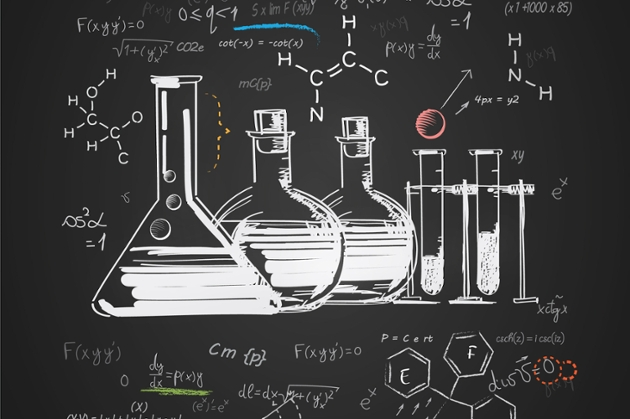
\includegraphics[width=0.9\textwidth]{chem1}
  \end{subfigure}%
  \begin{subfigure}[t]{0.45\textwidth}
    \centering
    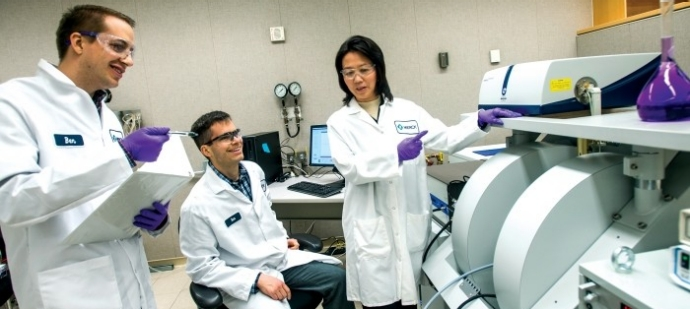
\includegraphics[width=0.9\textwidth]{chem2}
  \end{subfigure}\\
  \begin{subfigure}[t]{0.45\textwidth}
    \centering
    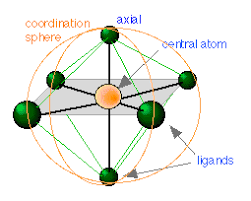
\includegraphics[width=0.9\textwidth]{chem3}
  \end{subfigure}%
  \begin{subfigure}[t]{0.45\textwidth}
    \centering
    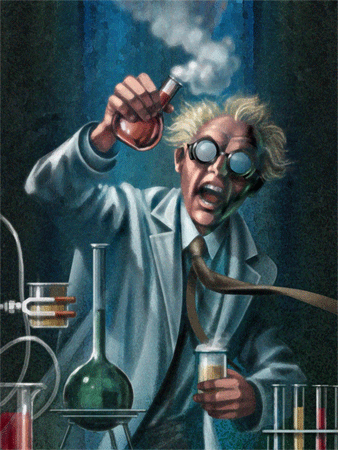
\includegraphics[width=0.9\textwidth]{chem4}
  \end{subfigure}\\
  \begin{subfigure}[t]{0.45\textwidth}
    \centering
    
\includegraphics[width=0.9\textwidth]{chem5}
  \end{subfigure}%
  \begin{subfigure}[t]{0.45\textwidth}
    \centering
    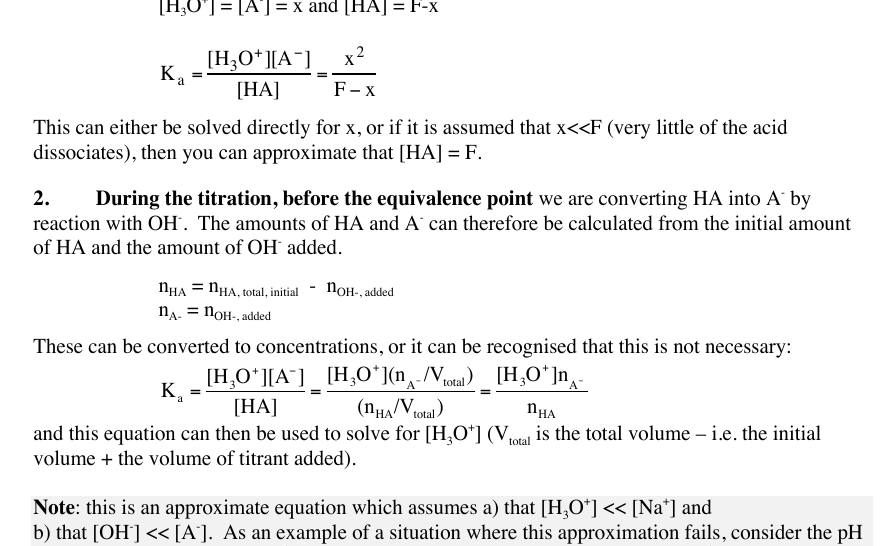
\includegraphics[width=0.9\textwidth]{chem6}
  \end{subfigure}
  \caption{Which picture best describes chemistry?\label{fig:chem}}
\end{figure}
\begin{center}
  \itshape
  Chemistry is the scientific discipline involved with compounds composed of atoms, i.e. elements, and molecules, i.e. combinations of atoms: their composition, structure, properties, behavior and the changes they undergo during a reaction with other compounds. (Wikipedia)
\end{center}

\begin{center}
  \itshape
  Studying chemistry will help you understand and appreciate the world in which you live. Advances in chemistry have had an enormous influence on our modern lifestyle and standard of living. Inventions such as semiconductors, polymers, pharmaceuticals and advanced materials of all kinds are based on chemical science. The study of chemistry leads to a deep appreciation of the scientific method, particularly the intellectual skills needed to develop new theories and to design experiments to test the validity of these theories. (Chemistry Undergrad. Handbook 2018, The Univ. of Auckland)
\end{center}

There are five main branches of chemistry; we'll look at each in turn.

\section{Analytical chemistry}
Analytical chemistry is the study of measurements.
\begin{itemize}
  \item How should we analyse compounds like pharmaceuticals?
  \item How do we know that our reaction produced what we think it did?
  \item How efficient is our process?
\end{itemize}
Essentially, an analytical chemist wants to find out what is in a given mixture, and how much of each component is present.

\section{Biochemistry}
Biochemistry is the branch of chemistry directly related to questions in biology.
\begin{itemize}
  \item How do biological processes function at a chemical level?
  \item How is evolution shaped through chemical processes?
\end{itemize}

\section{Inorganic chemistry}
Inorganic chemistry is the study of the makeup and reactions of inorganic compounds: any compound that is not composed mainly of carbon. Major
areas of study include metallic chemistry, nuclear chemistry, coordination chemistry, and industrial inorganic chemistry.
\begin{itemize}
  \item Why do the transition metals form brightly coloured solutions?
  \item Why do electrons sit where they do?
  \item What is the chemistry of uranium and other radioactive elements?
\end{itemize}

\section{Organic chemistry}
Organic chemistry is the theoretical side of biochemistry --- the study of carbon-containing compounds like oils, alcohols, and fats. Organic
chemists often work with massive molecules, including polymers like plastics.
\begin{itemize}
  \item How do we make biodegradable plastics?
  \item Can we make cleaner carbon-based fuels?
  \item How should we produce drugs efficiently?
\end{itemize}

\section{Physical chemistry}
Physical chemistry is the application of physics to chemistry. This includes the physical structure of molecules and atoms, as well as
electrochemistry and spectroscopy (the study of the interaction of molecules with light).
\begin{itemize}
  \item How can we build efficient batteries?
  \item How do superconductors work?
\end{itemize}

\chapter{Atoms and Molecules}
\section{Elements}
Every substance that you can see, hear, or touch is made of atoms. To a first approximation, the subject of chemistry is simply the
study of the properties of, and interactions between, atoms. Historically, the ancient Greeks postulated the existence of a smallest
unit of matter but it was not until the 19th century that experimental evidence of atoms was produced.

\begin{figure}
  \centering
  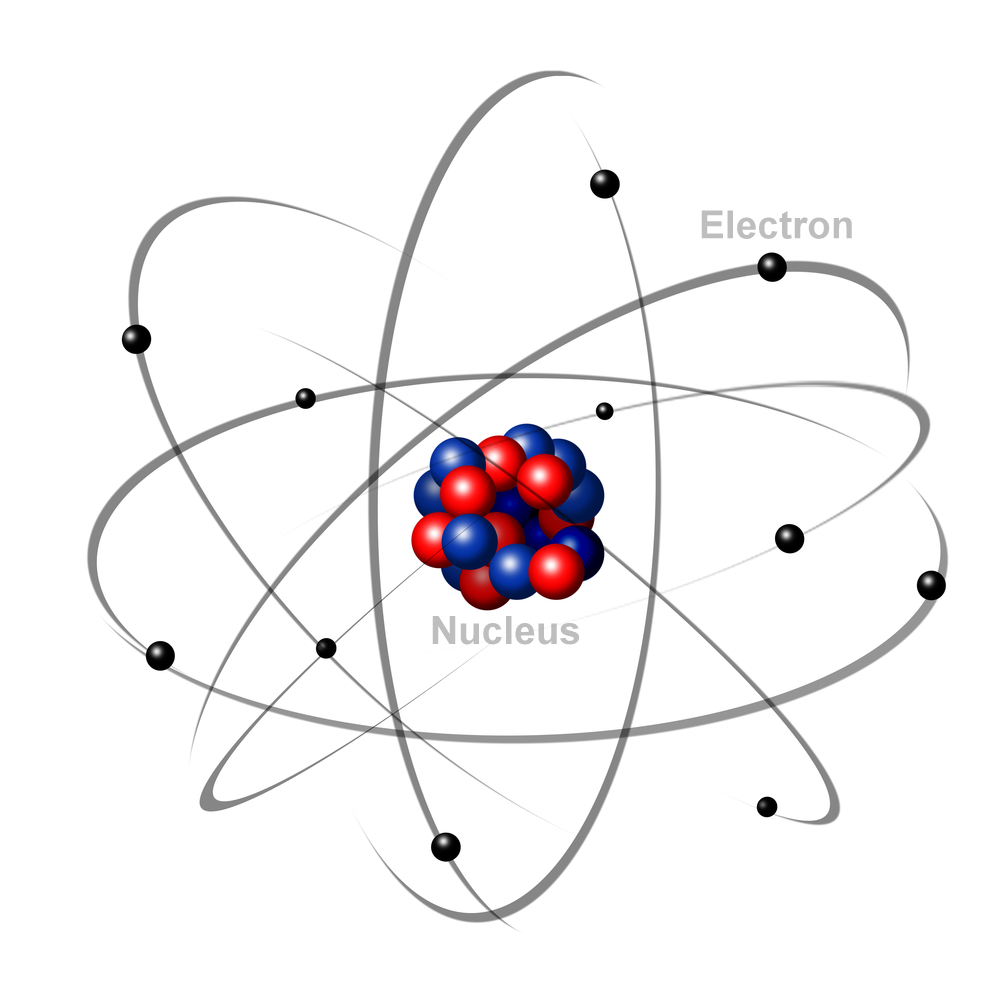
\includegraphics[width=0.5\textwidth]{atom}
  \caption{A diagram of an atom.\label{fig:atom}}
\end{figure}

An atom consists of a positively charged centre, called the nucleus, and a cloud of negatively charged electrons surrounding it. The nucleus is
futher made up of positively charged protons, and uncharged neutrons. Overall, an atom is electrically neutral: it has no net charge, because it
has the same number of protons as electrons. A simple model of the atom that is a good first approximation is given as \cref{fig:atom}.

A substance made up entirely of a single type of atom is called an element. Some examples of elements are shown as \cref{fig:elements}.

\begin{figure}
  \centering
  \begin{subfigure}[t]{0.45\textwidth}
    \centering
    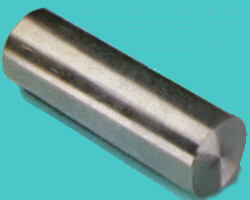
\includegraphics[width=0.9\textwidth]{uranium}
    \caption{Uranium metal.}
  \end{subfigure}%
  \begin{subfigure}[t]{0.45\textwidth}
    \centering
    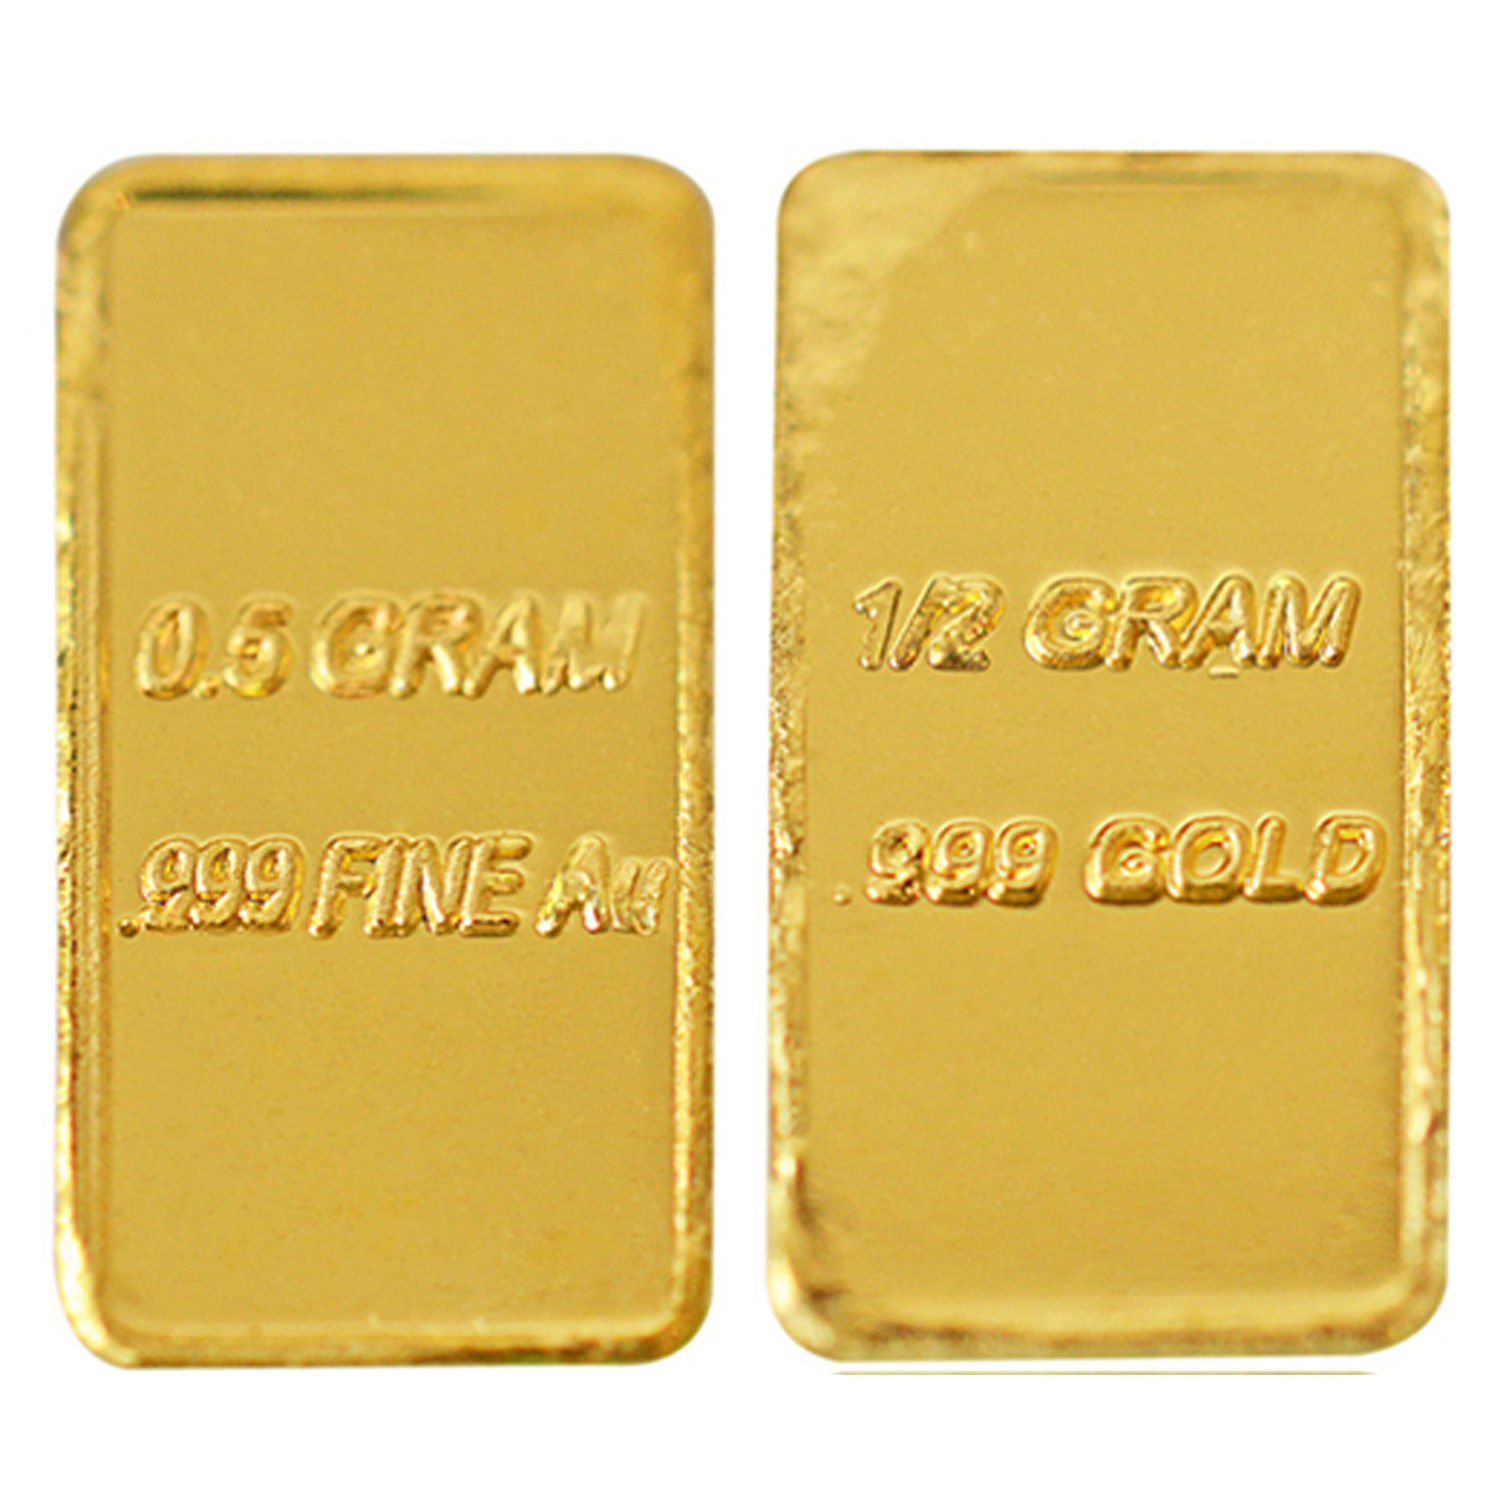
\includegraphics[width=0.9\textwidth]{gold}
    \caption{Gold metal.}
  \end{subfigure}\\
  \begin{subfigure}[t]{0.45\textwidth}
    \centering
    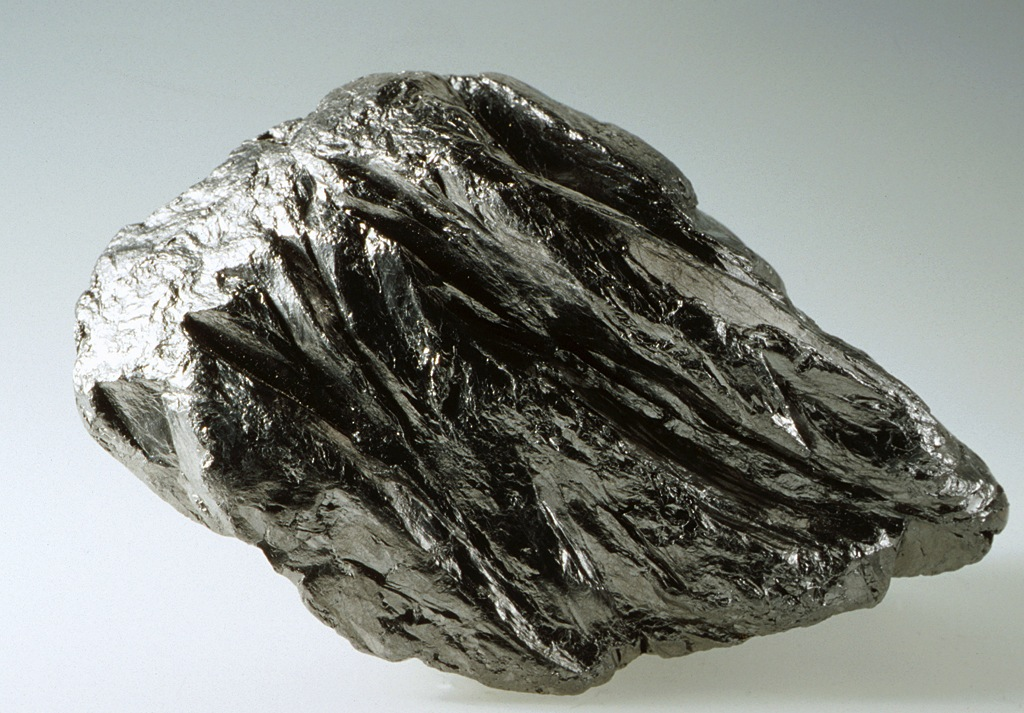
\includegraphics[width=0.9\textwidth]{graphite}
    \caption{Carbon, in the form of graphite.}
  \end{subfigure}%
  \begin{subfigure}[t]{0.45\textwidth}
    \centering
    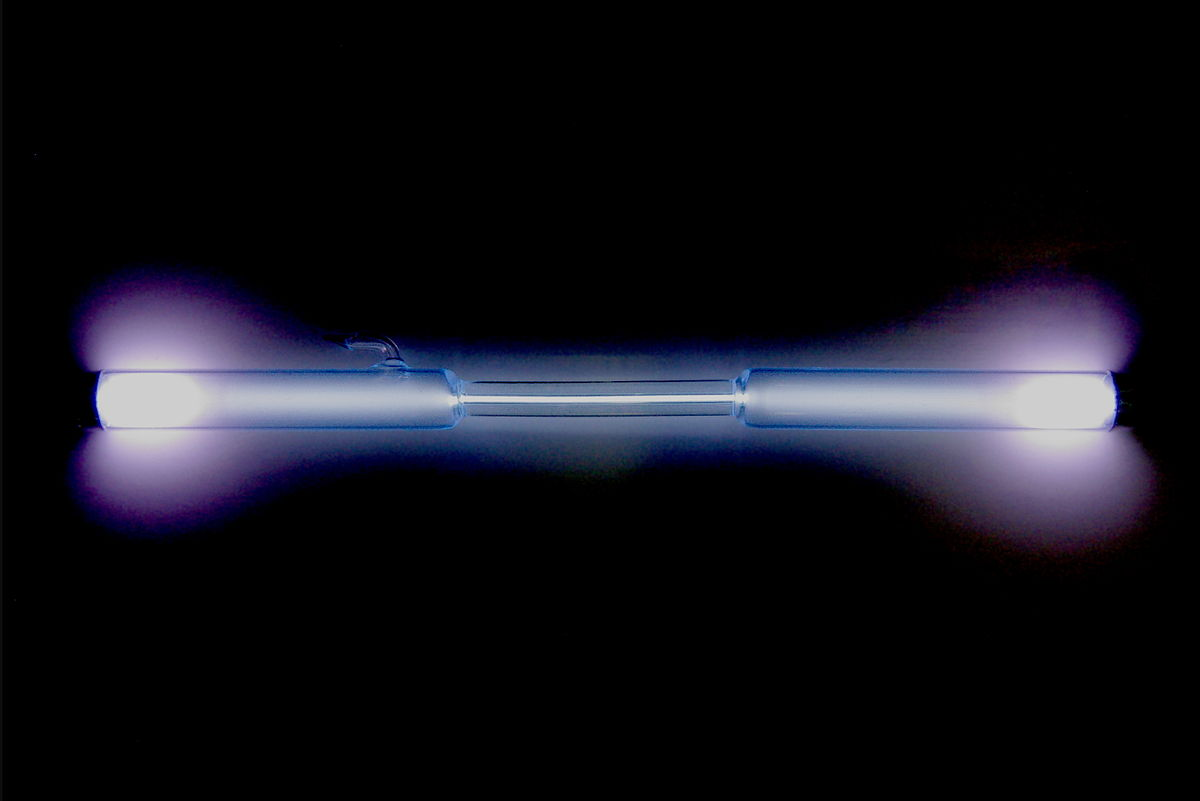
\includegraphics[width=0.9\textwidth]{xenon}
    \caption{Xenon gas is purple when an electric current passes through.}
  \end{subfigure}
  \caption{Four examples of elements.\label{fig:elements}}
\end{figure}

Different atoms have different properties depending on the number of protons in their nucleus; this number is called the atomic number of
the atom. The atom with atomic number 1 is hydrogen, a highly reactive gas. The atomic weight of an atom is the sum of the number of protons
and neutrons. Helium has two protons and two neutrons: it therefore has atomic number 2 and atomic weight 4. The type of the atom is entirely
determined by the atomic number --- every atom of boron has exactly five protons. However, not every atom of a particular element will always
have the same number of neutrons. For example, naturally occuring uranium can have 146, 143, or 142 neutrons. Different varieties of an element
with different atomic weights are called isotopes.

We can arrange the elements in a table, such that atoms in the same column have the same chemical properties: similar melting points, boiling
points, reactivities, and so on. We obtain what is called the periodic table of the elements, \cref{fig:ptable1}.\footnote{The reason that this
periodic table has non-integer atomic weights is that the weights given are an average of all the atomic weights of naturally occuring isotopes.
For example, carbon has two stable isotopes, \ce{^13 C} and \ce{^12 C}.} Each elementis given a symbol made up of one or two letters; for example,
maganese is \ce{Mn} and iodine is \ce{I}. Some elements, like gold (\ce{Au}), have symbols that appear unrelated to their names: this is usually
because the symbols are derived from the latin names for the elements.
\begin{itemize}
  \item Sodium (\ce{Ne}): the latin name is \textit{natrium}.
  \item Iron (\ce{Fe}): the latin name is \textit{ferrum}.
  \item Silver (\ce{Ag}): the latin name is \textit{argentum}.
  \item Tin (\ce{Sn}): the latin name is \textit{stannum}.
  \item Antimony (\ce{Sb}): the latin name is \textit{stibium}.
  \item Tungsten (\ce{W}): the symbol comes from the tungsten mineral wolfram.
  \item Mercury (\ce{Mg}): the symbol comes from the old name hydrargyrum.
  \item Lead (\ce{Pb}): the latin name is \textit{plumbum}.
\end{itemize}

\begin{figure}
  \centering
  \begin{sideways}
    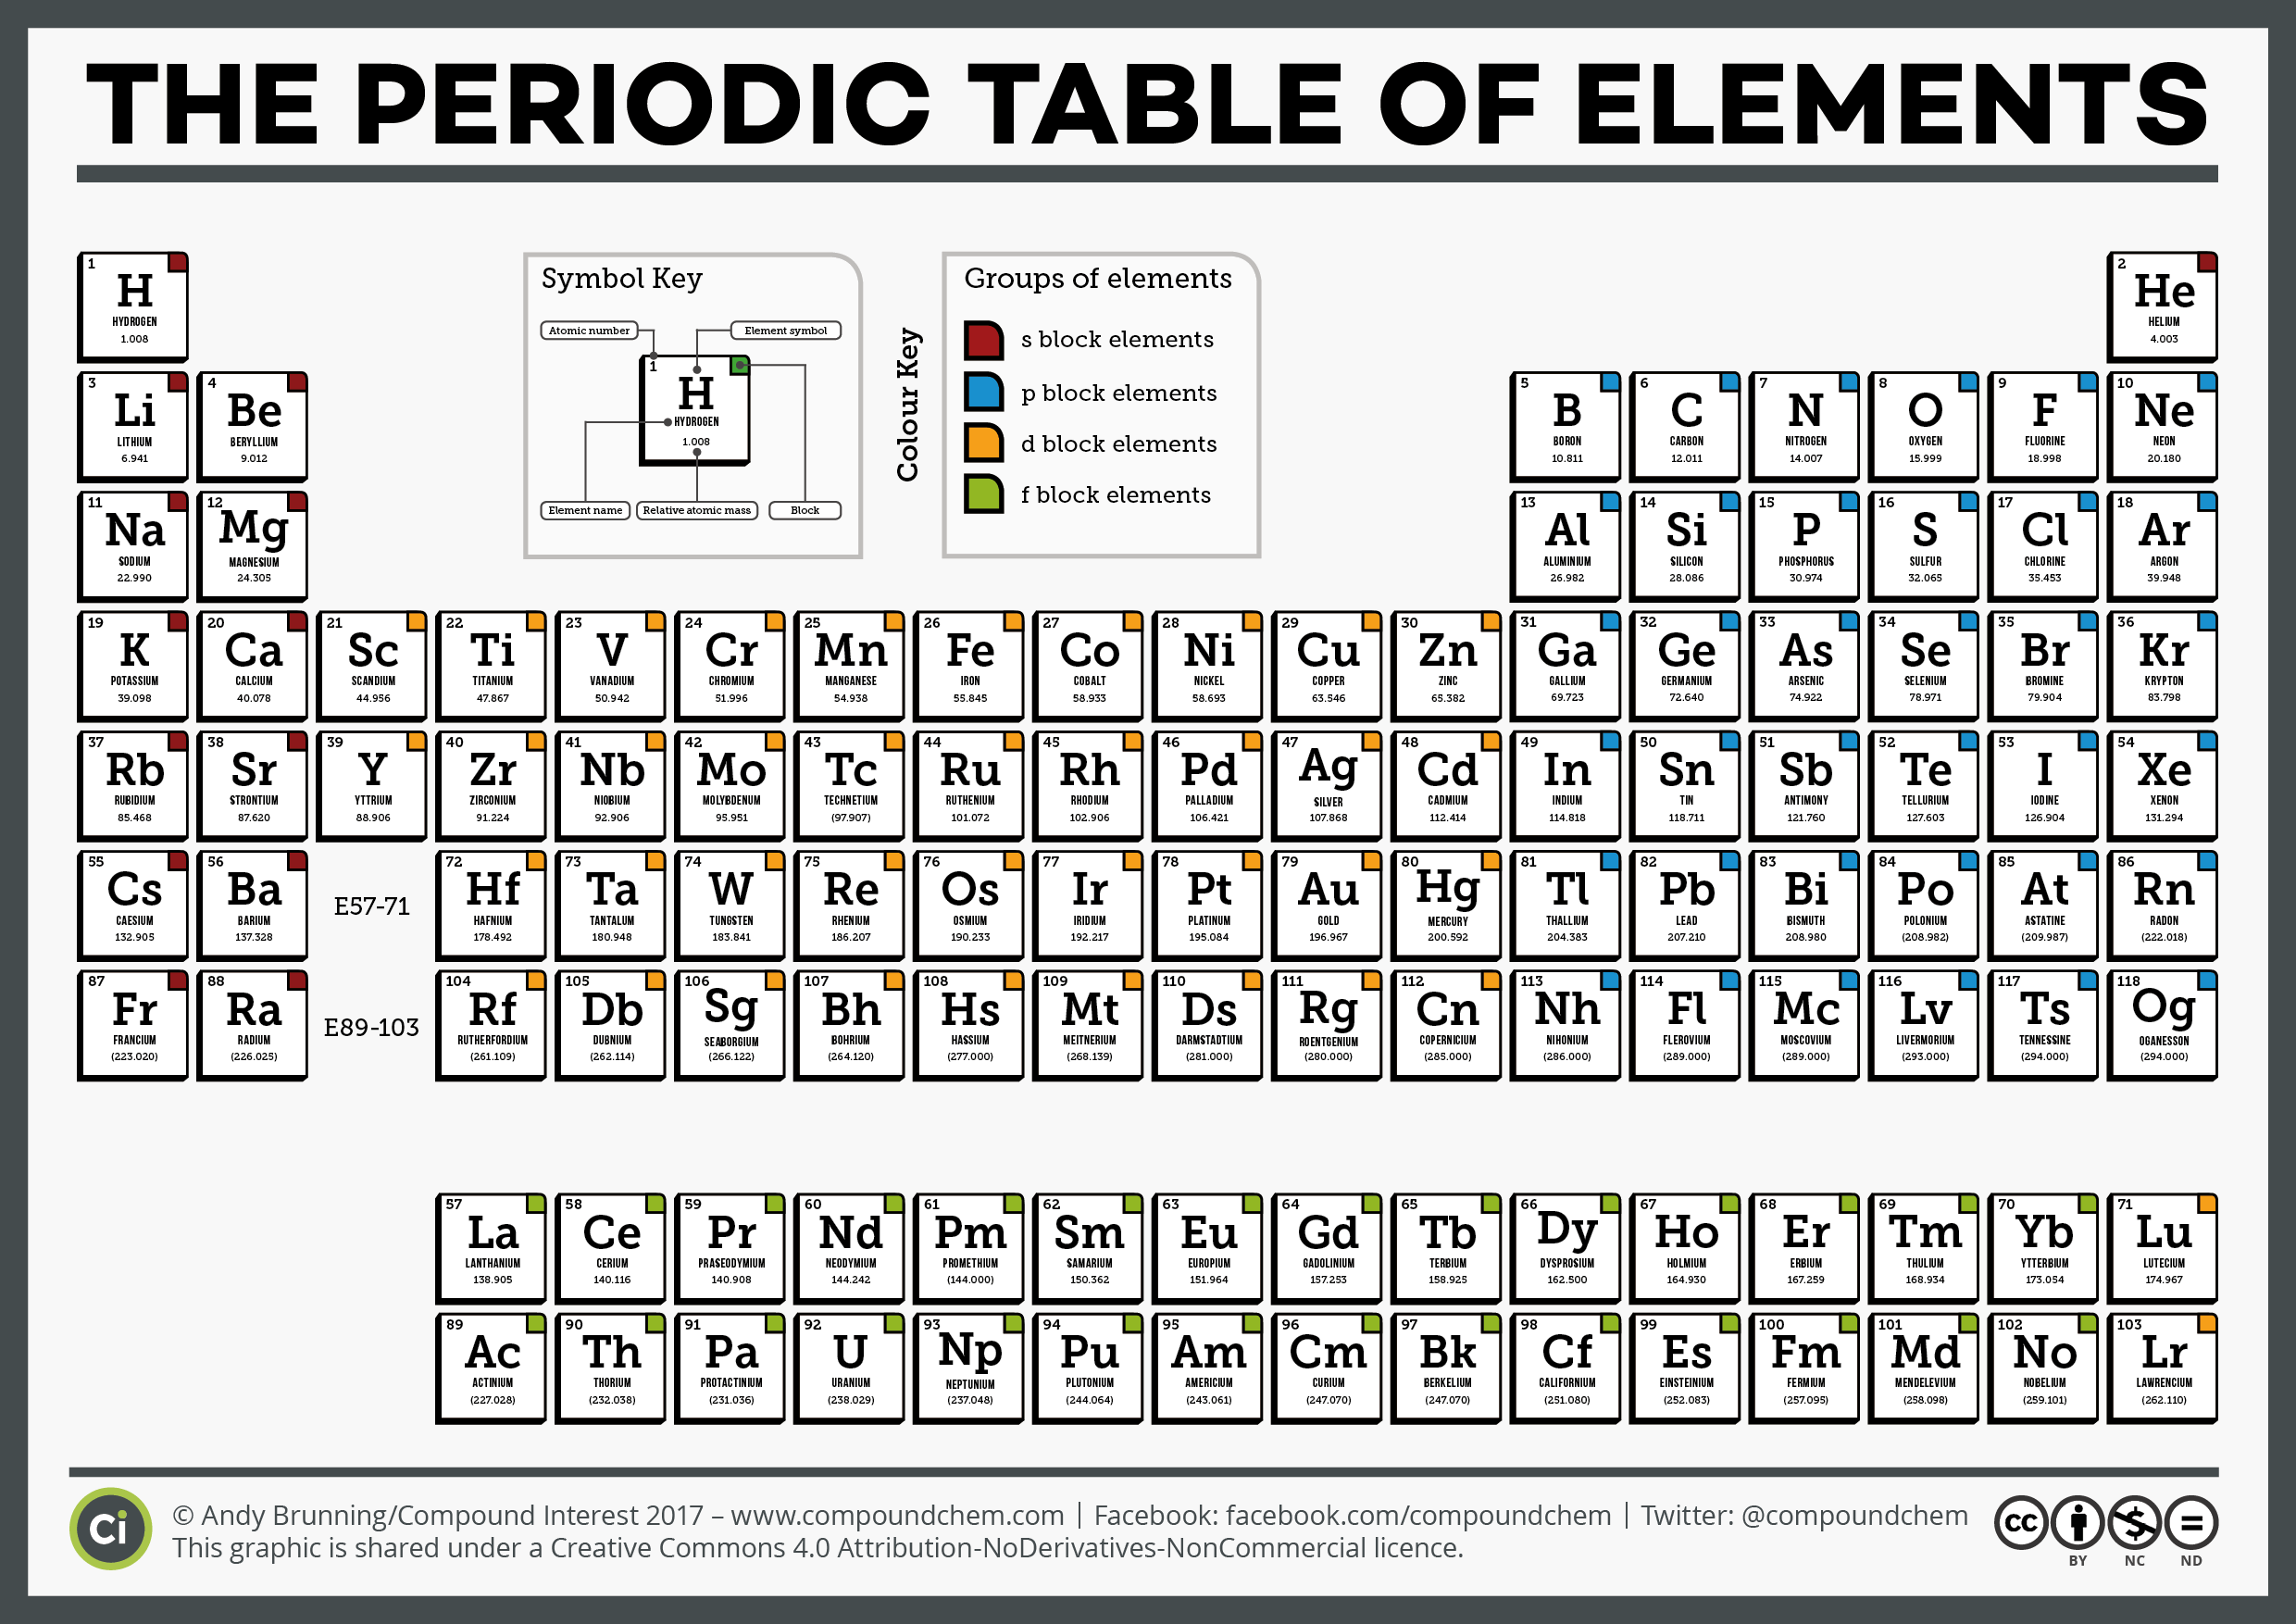
\includegraphics[height=1.2\textwidth]{ptable}
  \end{sideways}
  \caption{The periodic table.\label{fig:ptable1}}
\end{figure}

Some elements, like hydrogen and helium, do not exist naturally as single atoms; they bond in pairs, forming a molecule.

\begin{center}
  \chemfig{H-H}\\
  \chemfig{He-He}
\end{center}

Other atoms, like carbon, form massive three-dimensional structures. Graphite, a particular arrangement of carbon, is shown in \cref{fig:graphite2}.

\begin{figure}
  \centering
  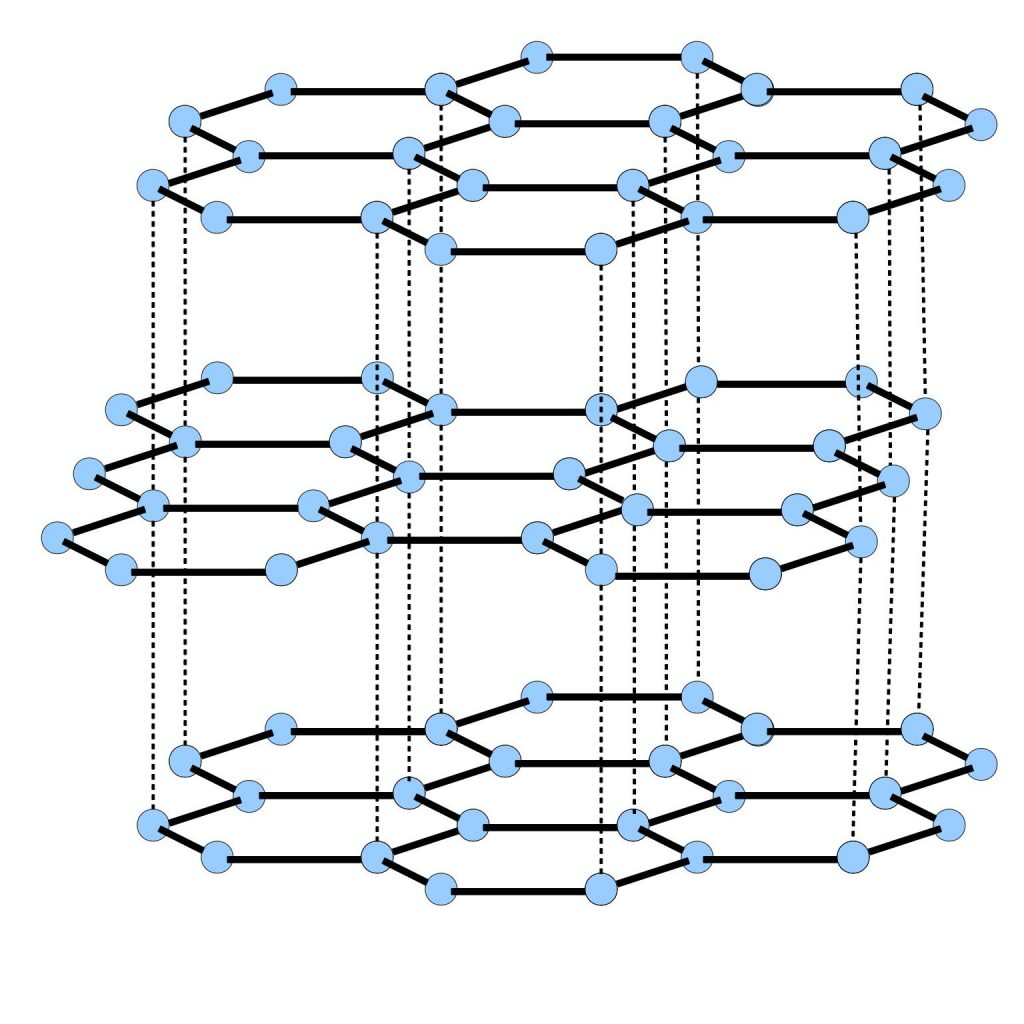
\includegraphics[width=0.5\textwidth]{graphite2}
  \caption{The physical structure of graphite. Blue dots represent carbon atoms.\label{fig:graphite2}}
\end{figure}

\subsection*{Exercises}
\begin{enumerate}
  \item ``Naturally occuring uranium can have 146, 143, or 142 neutrons.'' Give the atomic weight of each isotope of naturally occuring uranium.
  \item Consider the following elements: \ce{Be}, \ce{Mg}, \ce{Fe}, \ce{Nh}, \ce{In}, and \ce{W}. For each:
    \begin{enumerate}
      \item Give the elemental name.
      \item Give the atomic number.
      \item Rounding the atomic weights to the nearest whole number, calculate the number of neutrons and protons in the nucleus of the most
            common isotope.
    \end{enumerate}
\end{enumerate}

\section{Compounds}
Of course, not everything is an element. For example, the everyday substance that we call water does not appear on the periodic table anywhere. In
fact, water vapour can be formed by burning hydrogen gas in air; it turns out that water is made up of two atoms of hydrogen bonded to a single atom
of oxygen. The atomic formula of water is therefore \ce{H2O}.

\begin{center}
  \chemfig{H-[::37.78]O-[::-75.56]H}
\end{center}

A substance like water that is made up purely of a particular set of atoms bonded together in a particular way is called a compound. Some other simple
examples of compounds include carbon dioxide (made up of a carbon atom with two oxygen atoms), ammonia (made up of a nitrogen atom with three hydrogen
atoms); an example of a larger compound is chromium(II) acetate, with atomic formula \ce{C8H16Cr2O10} and displayed in \cref{fig:cr2ac}.

\begin{figure}
  \centering
  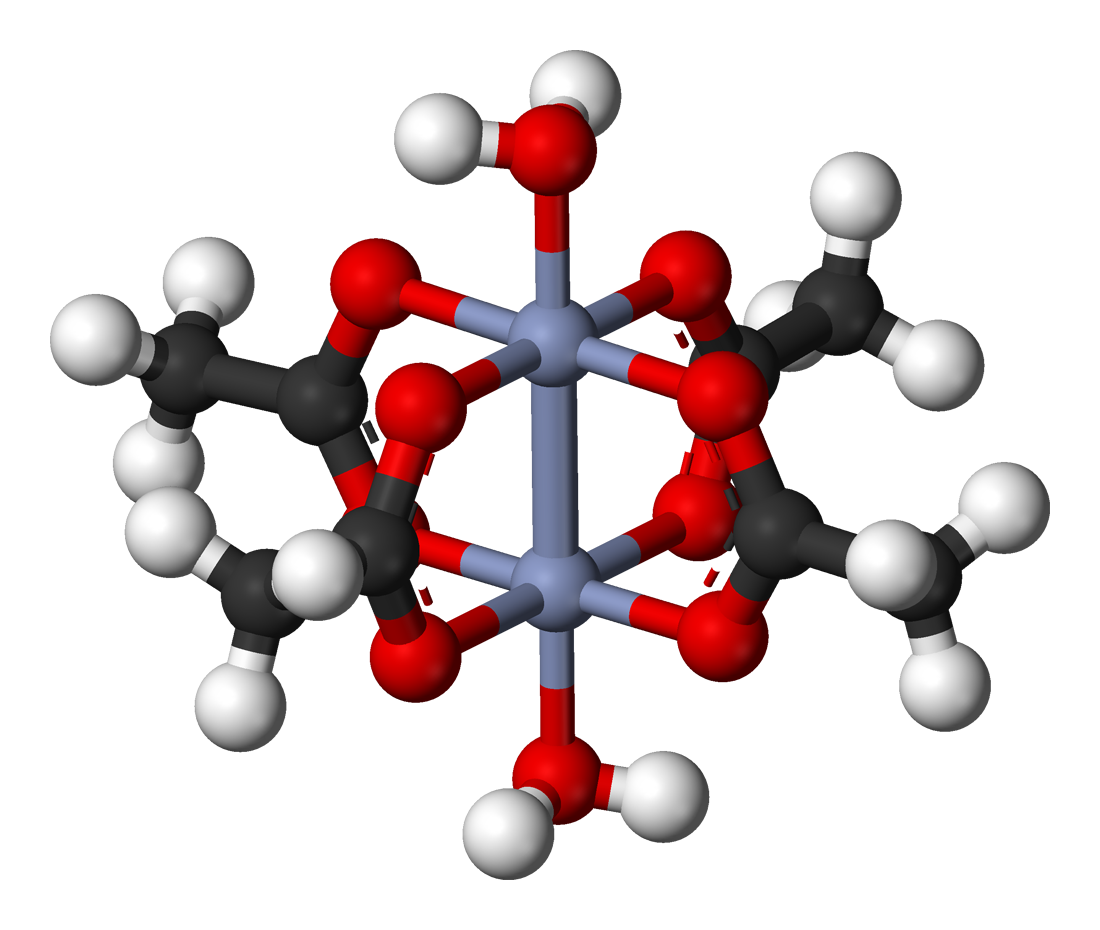
\includegraphics[width=0.5\textwidth]{cr2ac}
  \caption{A compound of dichromium. Blue: \ce{Cr}, red: \ce{O}, black: \ce{C}, grey: \ce{H}.\label{fig:cr2ac}}
\end{figure}

One of the primary tasks of chemistry is to explain why particular compounds are seen in nature, while others are not.

Some other compounds that you should be familiar with include:
\begin{itemize}
  \item Ammonia, \ce{NH3} (incredibly pungent gas, used as a precursor for foods, fertilisers, and pharmaceuticals).
  \item Calcium carbonate, \ce{CaCO3} (mineral found in rock).
  \item Sodium chloride, \ce{NaCl} (table salt).
  \item Sodium hypochlorate, \ce{NaClO} (used in bleach).
  \item Sodium hydroxide, \ce{NaOH} (also known as lye, used as drain cleaner).
  \item Ethanoic acid, \ce{CH3CHOOH} (active ingredient in vinegar).
\end{itemize}

As you can see, there are multiple ways to write down a chemical formula. Consider ammonia; it has
molecular formula \ce{NH3}, and we can draw its structural formula as well:
\begin{center}
  \chemfig{N(-[5]H)(-[6]H)(-[7]H)}
\end{center}

\subsection*{Exercises}
\begin{enumerate}
  \item Give the molecular formulae for the following molecules:
    \begin{enumerate}
      \item \chemfig{C(-[2]H)(-[4]H)(-[6]H)(-[0]H)}
      \item \chemfig{C(-[2]H)(-[4]H)(-[6]H)(-[0]OH)}
      \item \chemfig{Si(-[2]Cl)(-[4]Cl)(-[6]Cl)(-[0]Cl)}
    \end{enumerate}
  \item Ammonia is made up of nitrogen and hydrogen. Explain how ammonia gas is different from a mixture of nitrogen and hydrogen.
\end{enumerate}

\section{Ions}
Atoms are always electrically neutral. However, it is possible to force an atom to gain or lose an electron; the resulting charged particle is called
an ion. For example, we can remove the single electron from sodium, producing $ Na+ $.\footnote{It is even possible, though much harder, to add an electron
to sodium and form \ce{Na-}. The result is quite unstable.}

If we take a bunch of positive ions (cations) and negative ions (anions), they tend to want to clump together because opposite charges attract. A compound
made up of anions and cations bonded ionically is called a salt. Some examples of salts include table salt (\ce{NaCl}), hydrogen flouride (\ce{LiF}), and
magnesium chloride (\ce{MgCl2}). If a salt is placed in water, it will (usually) dissociate into its component ions; for example,
\begin{gather}
  \ce{NaCl ->[H2O] Na+ + Cl-}\\
  \ce{MgCl2 ->[H2O] Mg2+ + 2Cl-}
\end{gather}

You may have noticed that magnesium chloride is made up of two anions and only one cation. This is because elements in the main group of the periodic
table (up to element 20, calcium) are quite well-behaved: when they form ions, they gain or lose enough electrons to end up at the nearest noble gas (element
in the final column, like argon or neon). Why is this? It turns out that electrons tend sit at different orbits around the nucleus; let's take magnesium as
an example (\cref{fig:magnesiumshells}).

\begin{figure}
  \centering
  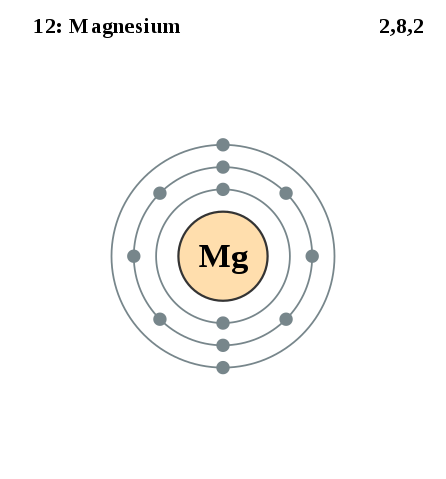
\includegraphics[width=0.5\textwidth]{magnesiumshells}
  \caption{The electron shells of a magnesium atom.\label{fig:magnesiumshells}}
\end{figure}

As you can see, the first two electrons sit the closest to the nucleus; then there is a second shell, which can fill up with the next eight electrons; and
in magnesium the third, outermost shell (the valence shell) fills up with the remaining two electrons. We say that the electron configuration of magnesium
is 2,8,2.

Another example is calcium (\cref{fig:calciumshells}), which has an electron configuration of 2,8,8,2.

\begin{figure}
  \centering
  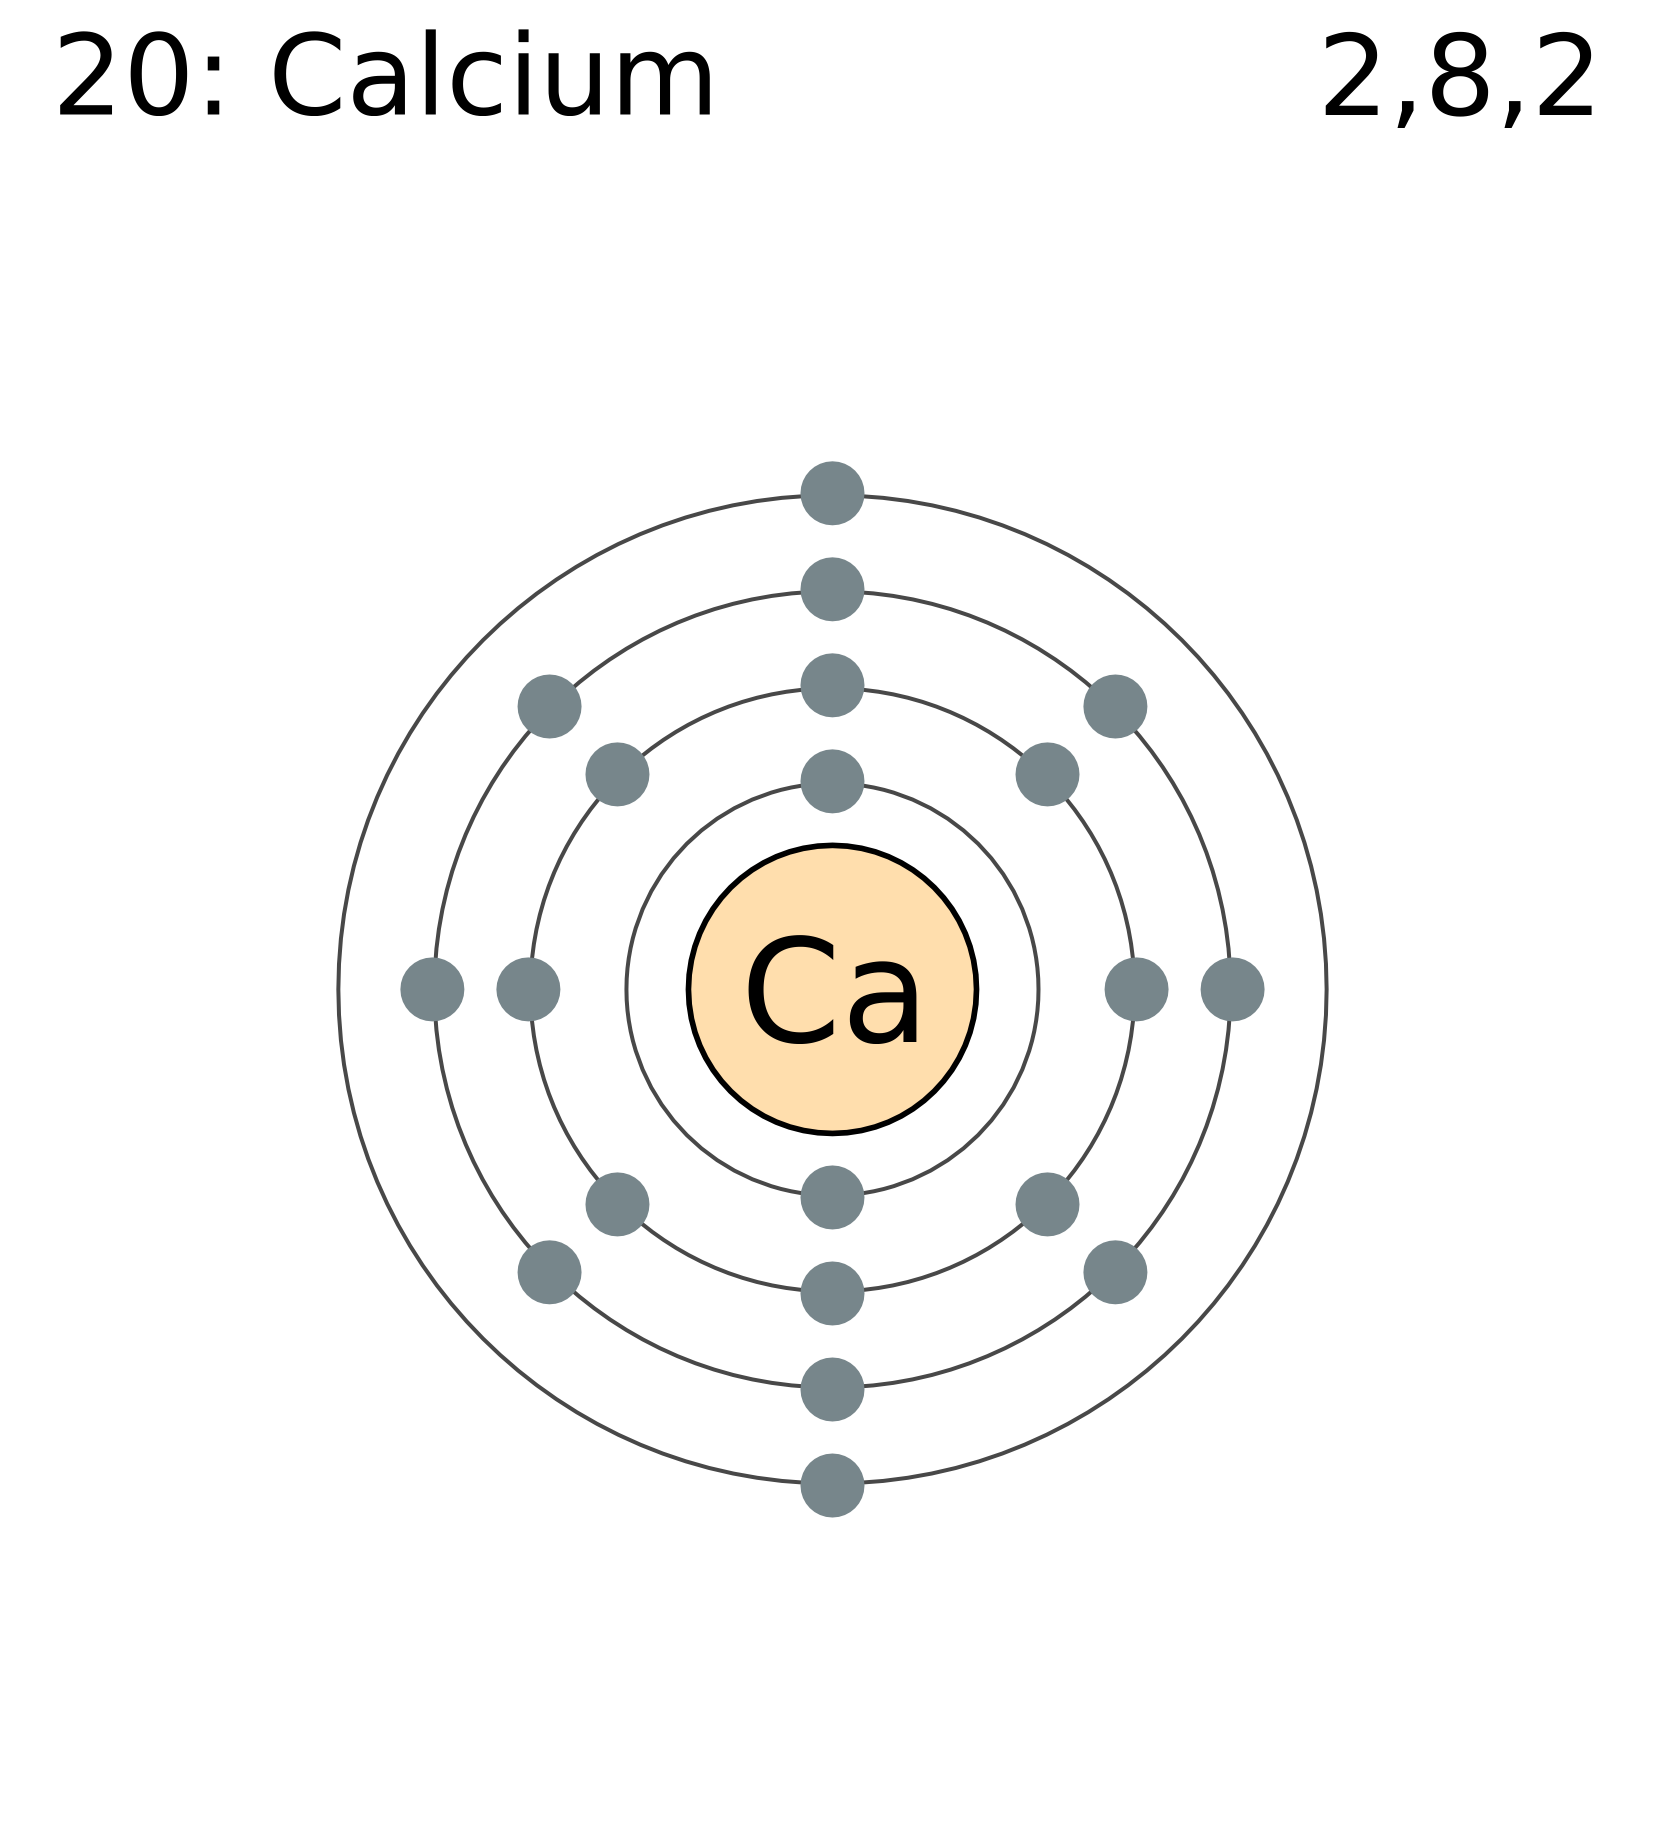
\includegraphics[width=0.5\textwidth]{calciumshells}
  \caption{The electron shells of a magnesium atom.\label{fig:calciumshells}}
\end{figure}

The electron structure of atoms can get much more complicated; however, there will always be two simple rules:
\begin{itemize}
  \item Atoms and ions with a full outer shell are very stable.
  \item Atoms and ions tend to want to gain or lose electrons in order to obtain a full outer shell.
\end{itemize}

Hence magnesium and calcium tend to want to lose their two valence electrons in order to obtain a full outer shell; chlorine and flourine
tend to want to gain an electron; and noble gases are incredibly stable, and so tend not to react with anything.\footnote{That's not to say
that they \emph{never} react: with some trouble it is possible to synthesise \ce{XeF4}, for example.}

\subsection*{Exercises}
\begin{enumerate}
  \item Give the electron configuration of the following atoms and ions:
    \begin{enumerate}
      \item \ce{Na+}
      \item \ce{B}
      \item \ce{Ar}
      \item \ce{Al^3+}
      \item \ce{O^2-}
      \item \ce{H+}
      \item \ce{H-}
    \end{enumerate}
  \item Explain why argon does not tend to form stable compounds.
  \item Give two examples of atom-like systems with the electron configuration 2,8.
  \item These chemicals are missing the correct subscripts; complete the formulae given.
    \begin{enumerate}
      \item \ce{Mg Cl_x}
      \item \ce{Al F_y} (in this compound, the aluminium ion has charge 3+)
      \item \ce{H_z Cl}
    \end{enumerate}
\end{enumerate}

\section{Covalent Bonds}
Atoms in the centre of the main group, like carbon and nitrogen, tend not to bond ionically because they are `too far' away from being ionic.
Instead, they tend to form covalent bonds: they share electrons with other atoms. Compounds made up of covalently bonded atoms and ions are
called molecules.

\begin{center}
  \chemfig{C(-[2]H)(-[4]H)(-[6]H)(-[0]H)}
\end{center}

Methane (\ce{CH4}) is an example of a covalently bonded molecule; it is also an example of an organic molecule (one which contains carbon). Each
bond consists of two electrons, shared between the carbon and hydrogen atoms.

\begin{center}
  \chemfig{C(-[2]H)(-[4]H)(-[6]H)-C(-[2]H)(-[6]H)-OH}
\end{center}

Ammonia, chlorine gas (\ce{Cl2}), oxygen gas, and ethanol (\ce{CH3CH2OH}) are also examples of covalently bonded molecules.

\begin{figure}
  \centering
  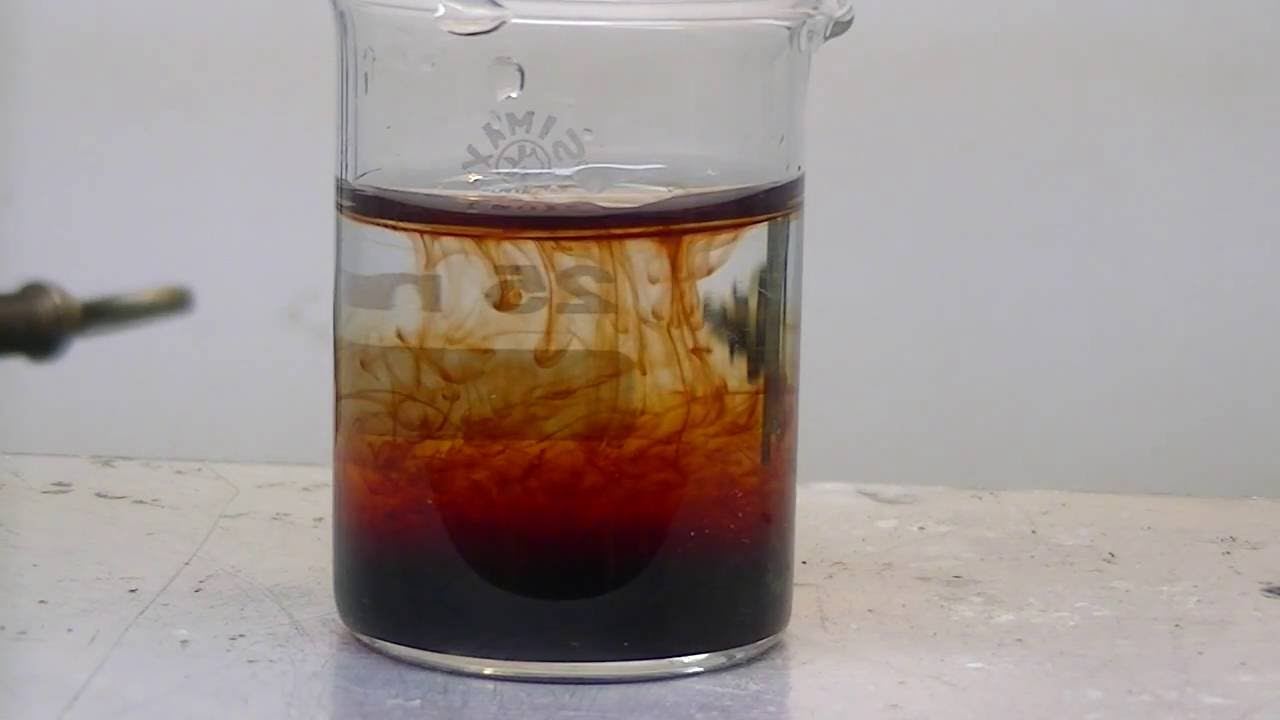
\includegraphics[width=0.8\textwidth]{thiocyanate}
  \caption{The formation of iron(III) thiocyanate from \ce{Fe3+} ions in solution.\label{fig:univindic}}
\end{figure}

Many covalent compounds are also ions. For example, the nitrate ion \ce{NO3-} consists of covalently bonded atoms; some others include:
\begin{itemize}
  \item Sulfate, \ce{SO4^2-}
  \item Hypochlorate, \ce{ClO-}
  \item Carbonate, \ce{CO3^2-}
  \item Hydrogen carbonate, \ce{HCO3^-}
  \item Iron(III) thiocyanate, \ce{[FeSCN(H2O)5]^{2+}} (\cref{fig:thiocyanate})
\end{itemize}

\subsection*{Exercises}
\begin{enumerate}
  \item Using your chemical knowledge, classify the following as ionic or covalent; if a substance is ionic, give the cation and anion.
    \begin{enumerate}
      \item Ethanol, \ce{CH3CH2OH}
      \item Sodium bromide, \ce{NaBr}
      \item Calcium carbonate
      \item Methane, \ce{CH4}
      \item Aluminium oxide
    \end{enumerate}
\end{enumerate}

\section{Chemical reactions}
The most interesting properties of elements and compounds come from their reactivities. A chemical reaction is a process which takes
a set of particles (the reactants) and rearranges the atoms and bonds to form a new set of particles (the products). We often summarise
a given reaction by writing a chemical equation:
\begin{equation}
  \ce{\text{products} -> \text{reactants}}
\end{equation}

For example, consider the following:
\begin{equation}
  \ce{CH2CH2 + Br2 -> CH2BrCH2Br}
\end{equation}
The corresponding word equation is:
\begin{equation}
  \ce{\text{ethene} + \text{bromide} -> \text{1,2-dibromo ethane}}
\end{equation}
From these equations, we see that in this reaction two molecules exchange bonds to form a single new molecule.

A chemical reaction can never create or destroy atoms, so the same number of each atom must occur on each side. In the following reaction,
multiple of the same molecule are needed to balance the equation:
\begin{equation}
  \ce{Mg + 2HCl -> H2 + Cl2}
\end{equation}

\chapter{Acids and Bases}
\section{Acid-base reactions}
We need the following definition:

{\itshape
  An \textbf{acid}\footnote{More specifically, a Br{\o}nsted-Lowry acid.} is a chemical species\footnote{A chemical species is any thing that
  exists on its own in solution --- for example, an ion or a molecule.} that tends to donate protons when in solution.
}

Recall that a proton is exactly the same thing as an \ce{H+} ion. An example of an acid is hydrogen chloride (usually known as hydrochloric acid), \ce{HCl}. In
water, it dissociates into ions:
\begin{equation}
  \ce{HCl ->[H2O] H+ + Cl-}
\end{equation}
In other words, the \ce{HCl} donates its proton into solution in the form of an \ce{H+} ion.\footnote{We're actually lying to you here: there is no such thing
as an \ce{H+} ion in water. In fact, the \ce{HCl} donates its proton to a water molecule which acts as a base, forming an hydronium ion (\ce{HCl + H2O -> H3O+ + Cl-}).}

Ammonia(\ce{NH3}), a colourless gas, also acts as an acid due to the following reaction:
\begin{equation}
  \ce{NH3 ->[H2O] NH2- + H+}
\end{equation}

A dual definition can also be made.

{\itshape
  A \textbf{base}\footnote{More specifically, a Br{\o}nsted-Lowry base.} (or an \textbf{alkaline species}) is a chemical species that tends to accept
  protons when in solution.
}

The main example of a base is the hydroxide ion \ce{OH-}; if it meets a proton swimming around in solution, it will combine with it to form a water molecule:
\begin{equation}
  \ce{OH- + H+ -> H2O}
\end{equation}

In reality, most of us do not keep a stock of hydroxide ions sitting around by themselves. Most bases that we use are salts that dissociate in water
to produce hydroxide ions, which then accept protons. Examples of bases include \ce{NaOH} and \ce{KOH}:
\begin{gather}
  \ce{NaOH ->[H2O] Na+ + OH-}\\
  \ce{KOH ->[H2O] K+ + OH-}
\end{gather}

Ammonia can also act as a base:\footnote{Water is another compound which can act as both an acid and a base.}
\begin{equation}
  \ce{NH3 + H+ -> NH4+}
\end{equation}

If we place sodium hydroxide and hydrochloric acid together in solution, the following set of reactions will occur:
\begin{gather*}
  \ce{NaOH ->[H2O] Na+ + OH-}\\
  \ce{HCl ->[H2O] H+ + Cl-}\\
  \ce{H+ + OH- -> H2O}\\
  \ce{Na+ + Cl- -> NaCl}
\end{gather*}
So in total, the following is observed:
\begin{equation}
  \ce{NaOH + HCl ->[H2O] NaCl + H2O}
\end{equation}

By the same reasoning, the following rule can be easily justified (where \ce{HA} is some acid, and \ce{BOH} is some base):
\begin{equation}
  \ce{HA + BOH -> AB + H2O}
\end{equation}
In other words, acid plus base forms salt plus water.

\subsection*{Exercises}
\begin{enumerate}
  \item Complete the following reaction schemes, making sure to balance where necessary:
    \begin{enumerate}
      \item \ce{H2SO4 + NaOH ->}
      \item \ce{HNO3 + CH3NH2 ->}
      \item \ce{HCl + KOH ->}
    \end{enumerate}
  \item Describe the reaction of ammonia with \ce{KOH}.
\end{enumerate}

\section{Measuring acidity}
\begin{figure}
  \centering
  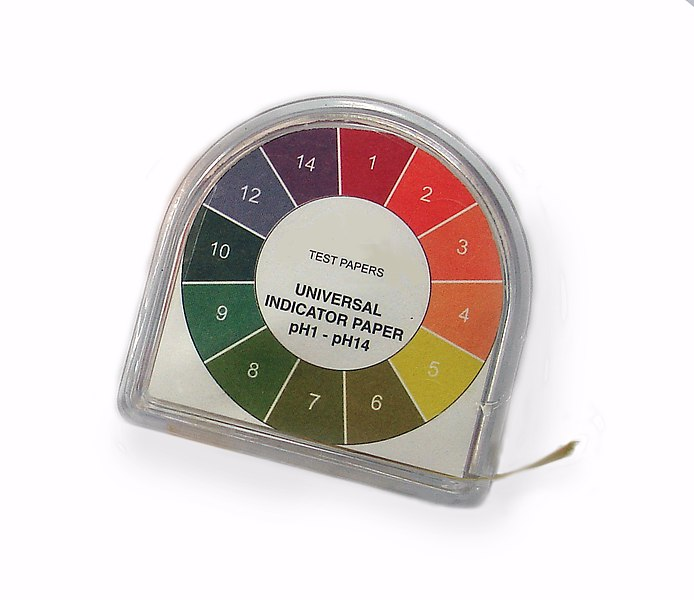
\includegraphics[width=0.8\textwidth]{univindic}
  \caption{The colours of universal indicator paper.\label{fig:univindic}}
\end{figure}

\begin{figure}
  \centering
  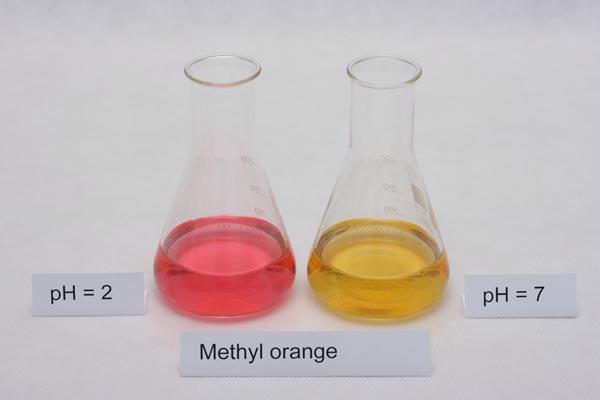
\includegraphics[width=0.8\textwidth]{methylorange}
  \caption{Another indicator is methyl orange; there are many others, and the choice of indicator depends on the particular
           reaction that is being carried out.\label{fig:methylorange}}
\end{figure}

\textbf{Important concept:} the strength of an acid is measured by the concentration of protons that it donates.

We measure the `acidity' of a solution using a scale known as the pH scale --- more acidic substances have a lower pH value. The acidity of a
substance can be measured by adding universal indicator and noting the colour change (\cref{fig:univindic}), by using litmus paper (acid turns blue
litmus paper red, and base turns red litmus paper blue), or by using an electronic pH meter.
\begin{center}
  \begin{tabular}{rlc}
    \textbf{pH value} & \textbf{Solution} & \textbf{Universal indicator colour}\\
    1 & \emph{(acidic)} \ce{HCl} & red\\
    2 & Lemon juice &\\
    3 & Ethanoic acid &\\
    6 & Milk, urine &\\
    7 & \emph{(neutral)} Pure water, blood & green\\
    8 & Sea water &\\
    9 & Baking soda (\ce{NaHCO3}) &\\
    11 & Ammonia &\\
    13 & \ce{NaOH} &\\
    14 & \emph{(basic)} \ce{H2SO4} & purple
  \end{tabular}
\end{center}

While most solutions you meet will have a pH in the range 1-14, it is important to realise that it is entirely possible to have a solution
with a pH outside that range; highly concentrated acids can have a negative pH value, for example.

\subsection*{Exercises}
\begin{enumerate}
  \item Chlorine water is formed by adding chlorine gas to water. Some of the chlorine dissolves in water and some reacts with water. Explain
        what happens to a piece of blue litmus paper when it is used to test the chlorine water.
  \item \ce{HCl} is sitting in aqueous solution. A small amount of universal indicator is added, and then sodium hydroxide is added dropwise.
        Describe and explain any observations.
\end{enumerate}

\section{Acid-metal reactions}

{\itshape
  A \textbf{metal} is an element that is shiny and generally hard when a solid, and is malleable (easy to bend), ductile (can be drawn into wires),
  and a good electrical conductor.\footnote{This is a very naive definition; more correctly, a metal is an element that has free valence electrons.}
}

If we drop a piece of metal into acid, then we observe bubbling on the surface of the metal. This is because the metal is donating electrons to the
acid, allowing the hydrogen cations to form covalent bonds and escape as a gas. Let's look at an example:
\begin{displaymath}
  \ce{Mg + 2HCl ->[H2O] MgCl2 + H2}
\end{displaymath}
Getting rid of the \ce{Cl-} anions that don't actually take part in the reaction, we have the following reaction:
\begin{equation}
  \ce{Mg + 2H+ -> Mg2+ + H2}
\end{equation}
We can split this up further, by looking at where the individual electrons go. There are two reactions happening at the same time:
\begin{gather}
  \ce{Mg -> Mg2+ + 2e-}\\
  \ce{2H+ + 2e- -> H2}
\end{gather}
This kind of reaction is an oxidation-reduction reaction (or redox reaction). This year, we only care about the specifics of acid/metal
reactions, but more interesting redox reactions can occur; for example, the underlying mechanism of a battery is a redox reaction.

In general, we have the unbalanced equation (where \ce{M} is a metal, and $ y $ is the absolute charge on the cation of \ce{M} that is formed)
\begin{equation}
  \ce{M + 2H+ -> M^y- + H2}
\end{equation}
In other words, metal plus proton gives metal ion plus hydrogen (or metal plus base gives salt plus hydrogen). One final balanced example:
\begin{equation}
  \ce{Zn + 2HCl -> ZnCl2 + H2} \text{ (see \cref{fig:zncl})}
\end{equation}

Note that usually energy is released from a metal/acid reaction as heat.

\begin{figure}
  \centering
  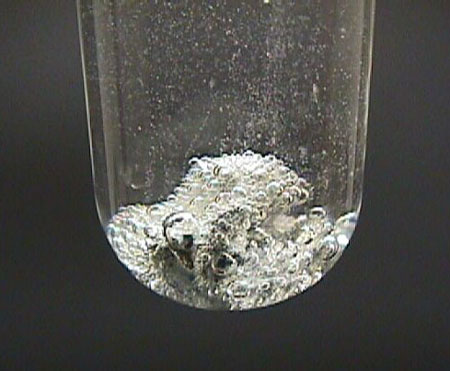
\includegraphics[width=0.5\textwidth]{zncl}
  \caption{The reaction of zinc metal with hydrochloric acid.\label{fig:zncl}}
\end{figure}

Acids also react with metal oxides. For example,
\begin{equation}
  \ce{MgO + 2HNO3 ->[H2O] H2O + Mg(NO3)2}
\end{equation}

In general, a metal oxide plus an acid produces a salt and water.

\subsection*{Exercises}
\begin{enumerate}
  \item Small pieces of zinc were dropped into a test tube of dilute sulfuric acid solution. Describe the observations you would make of this reaction.
  \item Magnesium is added to nitric acid. Write down a balanced equation for this reaction.
\end{enumerate}

\section{Acid-carbonate reactions}
Carbonates and hydrogen carbonates also react with acids. Like with metals, a gas is produced; however, this time it is carbon
dioxide (\ce{CO2}) that is produced. Two examples:
\begin{gather}
  \ce{NaHCO3 + HCl ->[H2O] NaCl + H2O + CO2}\\
  \ce{MgCO3 + H2SO4 ->[H2O] MgSO4 + H2O + CO2}
\end{gather}

Again, this is an example of a redox reaction.

\begin{figure}
  \centering
  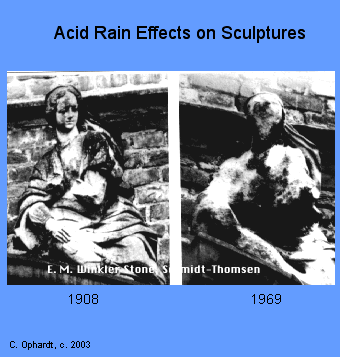
\includegraphics[width=0.5\textwidth]{acidrain}
  \caption{The effect of acid rain on a sculpture.\label{fig:acidrain}}
\end{figure}

\subsection*{Exercises}
\begin{enumerate}
  \item Limestone is primarily made up of calcium carbonate. When acid rain (containing a component of sulfuric acid) falls on sculptures or buildings built
        of limestone, what would you expect to observe over time? (\cref{fig:acidrain})
  \item Explain why eggshells soften in vinegar.
\end{enumerate}


\chapter{Solubility and States of Matter}
\section{Solutions}
\begin{figure}
  \centering
  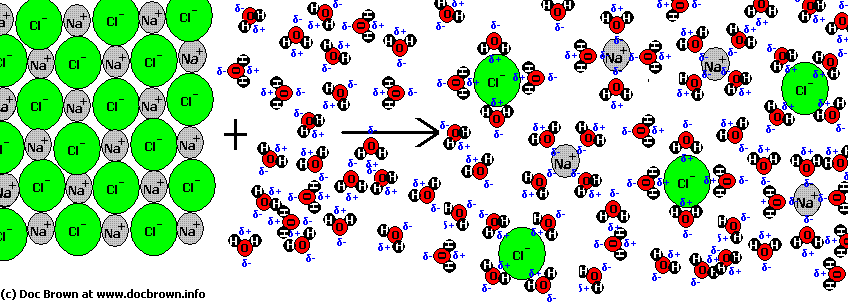
\includegraphics[width=\textwidth]{dissolving}
  \caption{The dissolution of table salt in water.\label{fig:dissolving}}
\end{figure}
A solution is a mixture of two substances, such that one substance (the solute) is dissolved in the other (the solvent). Common solvents
include water and ethanol.

Most salts are highly soluble (dissolve easily) in water, because water is polar --- water molecules have one end with a slightly negative charge
and one end with a slightly positive charge, so positive ions and negative ions are attracted to different ends of the water molecules and so are
split up. A diagram showing this process for \ce{NaCl} is given as \cref{fig:dissolving}; the negative ends of the water molecules are marked by $ \delta^- $,
and the positive ends by $ \delta^- $.

At room temperature, we have the following solubility rules for salts:

\begin{tabular}{ll}
  Nitrates (\ce{NO3-}) & All soluble\\
  Chlorides (\ce{Cl-}) & All soluble except \ce{AgCl} and \ce{PbCl2}\\
  Iodides (\ce{I-}) & All soluble except \ce{AgI} and \ce{PbI2}\\
  Sulphates (\ce{SO4^2-}) & All soluble except \ce{BaSO4}, \ce{PbSO4}, and \ce{CaSO4}\\
  Hydroxides (\ce{OH-}) & All insoluble except \ce{KOH} and \ce{NaOH}\\
  Carbonates (\ce{CO3^2-}) & All insoluble except \ce{K2CO3} and \ce{Na2CO3}\\
\end{tabular}

It is important to realise that all compounds are soluble to some degree; calcium carbonate (limestone, \ce{CaCO3}) is insoluble in water according to
the rules above, but this means that very little compound will dissolve --- not none! Conversely, even if a compound is highly soluble there is a maximum
amount that can be held in solution: if one continues to add salt to water, eventually it will cease to dissolve. A solution containing the maximum amount
of solute for the given temperature and amount of solvent is called saturated.

The solubility of a solute can be increased by:
\begin{itemize}
  \item Increasing the temperature of the solvent. (Warm water dissolves more solvent.)
  \item Reducing the common-ion effect (e.g. if \ce{NaOH} is added to a solution that already contains \ce{OH-} ions, then
        it has reduced solubility; conversely, removing \ce{OH-} ions will increase the solubility of \ce{Na+} ions from the \ce{NaOH}).
  \item Increasing pressure on the solution (if we are trying to dissolve a gas like \ce{HCl}).
\end{itemize}

\subsection*{Exercises}
\begin{enumerate}
  \item Classify as soluble or insoluble in water:
    \begin{enumerate}
      \item \ce{KI}
      \item \ce{KNO3}
      \item \ce{Pb(OH)2}
      \item \ce{Ag2SO4}
      \item \ce{CaCO3}
    \end{enumerate}
\end{enumerate}

\section{States of Matter}
\begin{figure}
  \centering
  \begin{subfigure}[t]{\textwidth}
    \centering
    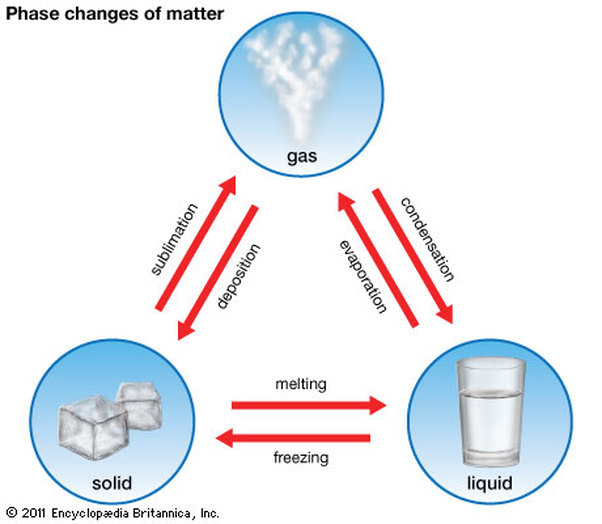
\includegraphics[width=0.8\textwidth]{states1}
    \caption{Transitions between states.}
  \end{subfigure}\\
  \begin{subfigure}[t]{\textwidth}
    \centering
    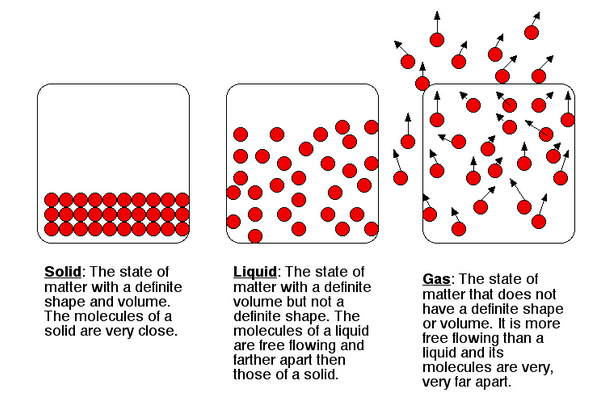
\includegraphics[width=0.8\textwidth]{states2}
    \caption{Physical properties of states.}
  \end{subfigure}
  \caption{The three common states of matter. \label{fig:states}}
\end{figure}
Obviously the behaviour of substances when we try to dissolve them depends on the state which they are in: solid, liquid, or gas (\cref{fig:states}). When
we write chemical equations, we place the state of each product and reactant in brackets behind them: \ce{(s)} --- solid; \ce{(\ell)} --- liquid;
\ce{(g)} --- gas;  \ce{(aq)} --- aqueous (in solution with water, like \cref{fig:dissolving}).\footnote{One may also see \ce{(alc)}, for substances dissolved
in ethanol or other alcohols.}

Let's look at a few examples of equations:
\begin{gather}
  \ce{NaCl(s) ->[H2O] Na+(aq) + Cl-(aq)}\\
  \ce{NH3(g) + H2O(\ell) -> NH2-(aq) + H3O+(aq)}\\
  \ce{AgBr(s) + KI(s) ->[H2O] AgI(s) + K+(aq) + Br-(Aq)}
\end{gather}

\begin{figure}
  \centering
  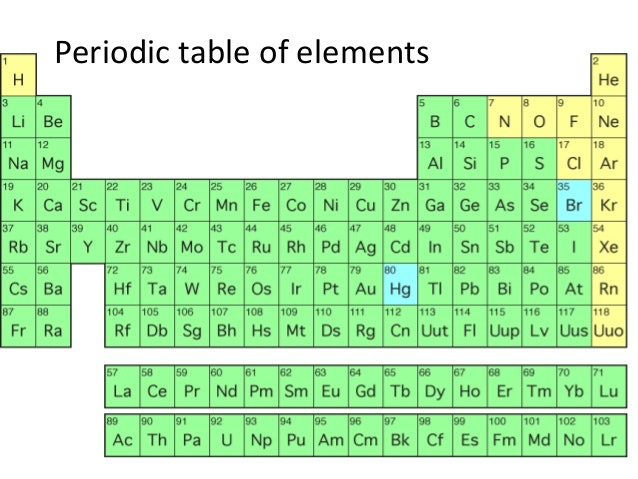
\includegraphics[width=0.7\textwidth]{ptable2}
  \caption{The periodic table by state (green: solid, yellow: gas, red: liquid).\label{fig:ptable2}}
\end{figure}

\begin{figure}
  \centering
  \begin{subfigure}[t]{0.45\textwidth}
    \centering
    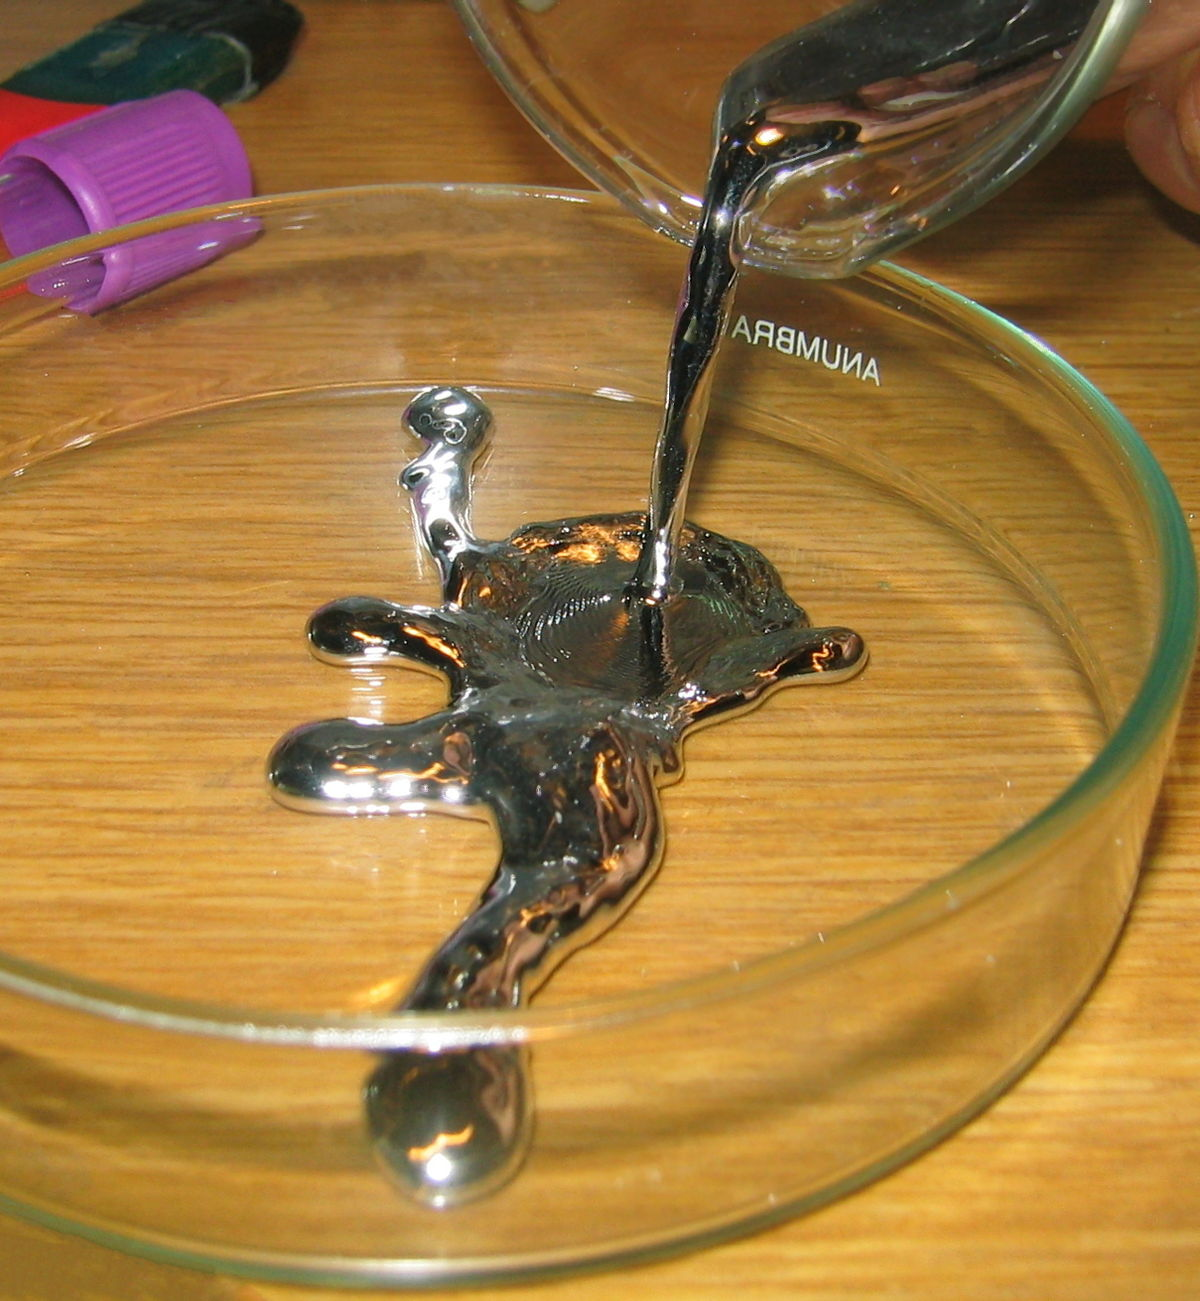
\includegraphics[width=0.9\textwidth]{mercury}
    \caption{Liquid mercury.}
  \end{subfigure}%
  \begin{subfigure}[t]{0.45\textwidth}
    \centering
    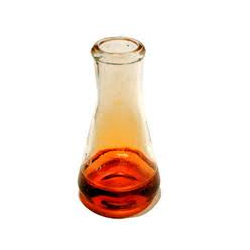
\includegraphics[width=0.9\textwidth]{bromine}
    \caption{Liquid bromine.}
  \end{subfigure}
  \caption{The only two elements which are liquid at room temperature. \label{fig:merbro}}
\end{figure}

In order to change matter from one state to another, we must either put energy in or take energy out. A process which requires energy to be input
to occur is called endothermic; a process which outputs energy is called exothermic. Melting and evaporation are endothermic processes, because we need
to input energy into the system to make them happen; condensation and freezing are exothermic processes, because energy is released by the system when
they occur.

There are, in fact, four fundamental states of matter: apart from solid, liquid, and gas, one can produce plasma (a state in which the electrons are ripped
entirely free from the nucleus) by heating gas. Plasma is generated when lightning strikes, and within neon lights. Nuclear fusion normally takes place
in a plasma of $ ^2H $ and $ ^3H $, like that found in the sun.

We can classify the elements by their state at room temperature (\cref{fig:ptable2}). Most elements are solid; the noble gases and some other elements in the
upper right portion of the table are gaseous at room temperature; and only two elements (mercury and bromine, \cref{fig:merbro}) are liquid.

\subsection*{Exercises}
\begin{enumerate}
  \item Add the states of matter to the following equations:
    \begin{enumerate}
      \item \ce{2NaCl + 2H2O -> 2NaOH + H2 + Cl2}
      \item \ce{H+ + OH- -> H2O}
      \item \ce{Mg + 2HCl -> H2 + MgCl2}
    \end{enumerate}
  \item Classify the following as exothermic or endothermic:
    \begin{enumerate}
      \item Sublimation.
      \item Deposition.
      \item Cooking an egg.
      \item Reacting an acid with a metal.
    \end{enumerate}
\end{enumerate}

\chapter{Rates of Reaction}
\section{Collision theory}
One model of chemical reactions is collision theory. According to this model, reactants can combine to form products if:
\begin{itemize}
  \item The reactant particles collide with enough energy (the activation energy); and
  \item The reactant particles collide in the correct orientation.
\end{itemize}

Graphical depictions of these requirements for a successful collision and therefore reaction can be seen in \cref{fig:collision}.

\begin{figure}
  \centering
  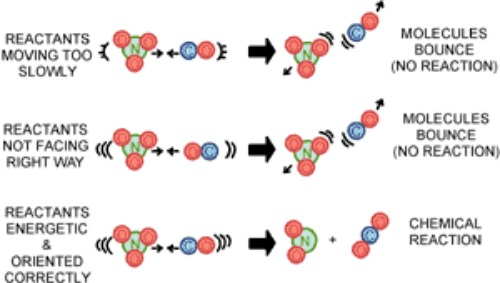
\includegraphics[width=0.8\textwidth]{collision}
  \caption{Collision theory.\label{fig:collision}}
\end{figure}

It immediately follows that in order to increase the rate of a reaction, we can take the following steps:
\begin{itemize}
  \item Increase the concentration of the reactants and/or increase the pressure of any gaseous reactants (so that the frequency
        of particle collisions is increased, and hence more successful collisions occur per second).
  \item Increase the temperature of the reactants (so that the speed of particles is increased, and more collisions occur with
        enough energy).
  \item Add a catalyst to the reaction (which provides an alternate reaction pathway with lower activation energy).
  \item Increase the surface area of any reactants in solid form (so that more reactant particles are exposed, and collisions
        can occur more frequently).
\end{itemize}

\section{Catalysts and reaction profiles}
\begin{figure}
  \centering
  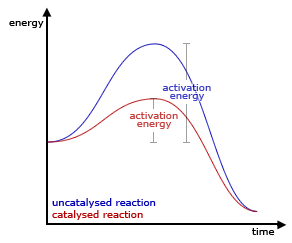
\includegraphics[width=0.5\textwidth]{catalyst}
  \caption{A reaction profile with and without a catalyst.\label{fig:catalyst}}
\end{figure}

A reaction is exothermic if the total amount of energy of the products is less than the total amount of energy of the reactants. This
energy is stored in the bonds between the atoms in the compounds, and is known as enthalpy.

In order for a reaction to occur, some energy must be provided to `get it going' --- this is the activation energy mentioned above. The
two diagrams in \cref{fig:catalyst} show the enthalpy stored in a given system during a reaction; since the energy of the reactants
is less than the energy of the products, the reaction is exothermic.

The diagram also shows the action of a catalyst. Reactions usually occur in steps, producing intermediate products (like carbocations) by
moving electrons around; a catalyst simply enables a different pathway of intermediate steps that requires a lower activation energy
than the non-catalysed reaction path. Catalysts are not used up in reactions.

Some examples of catalysts:
\begin{itemize}
  \item Platinum is used in car exhausts as a catalyst to break down some nasty products of combustion: \ce{2CO + 2NO ->[Pt] 2CO2 + N2}.
  \item Chlorine free radicals (\ce{Cl^{.}}, a chlorine atom that has lost a particular electron) are formed by the action of UV light
        on chlorofluorocarbons, and catalyse the breakdown of ozone through the following pair of reactions: \ce{Cl^. + O3 -> ClO^. + O2}
        and \ce{ClO^. + O -> Cl^. + O2} (so the observed reaction is \ce{O3 + O ->[Cl^.] 2O2}).
  \item Polypropylene is produced using a titanium-based catalyst.
\end{itemize}

\end{document}
